% Options for packages loaded elsewhere
\PassOptionsToPackage{unicode}{hyperref}
\PassOptionsToPackage{hyphens}{url}
%
\documentclass[
  12pt,
]{article}
\title{Impacts of Dam Removal on the Shenandoah River}
\usepackage{etoolbox}
\makeatletter
\providecommand{\subtitle}[1]{% add subtitle to \maketitle
  \apptocmd{\@title}{\par {\large #1 \par}}{}{}
}
\makeatother
\subtitle{\url{https://github.com/lydiecos/WDA-Dam-Removal}}
\author{Lydie Costes}
\date{}

\usepackage{amsmath,amssymb}
\usepackage{lmodern}
\usepackage{iftex}
\ifPDFTeX
  \usepackage[T1]{fontenc}
  \usepackage[utf8]{inputenc}
  \usepackage{textcomp} % provide euro and other symbols
\else % if luatex or xetex
  \usepackage{unicode-math}
  \defaultfontfeatures{Scale=MatchLowercase}
  \defaultfontfeatures[\rmfamily]{Ligatures=TeX,Scale=1}
  \setmainfont[]{Times New Roman}
\fi
% Use upquote if available, for straight quotes in verbatim environments
\IfFileExists{upquote.sty}{\usepackage{upquote}}{}
\IfFileExists{microtype.sty}{% use microtype if available
  \usepackage[]{microtype}
  \UseMicrotypeSet[protrusion]{basicmath} % disable protrusion for tt fonts
}{}
\makeatletter
\@ifundefined{KOMAClassName}{% if non-KOMA class
  \IfFileExists{parskip.sty}{%
    \usepackage{parskip}
  }{% else
    \setlength{\parindent}{0pt}
    \setlength{\parskip}{6pt plus 2pt minus 1pt}}
}{% if KOMA class
  \KOMAoptions{parskip=half}}
\makeatother
\usepackage{xcolor}
\IfFileExists{xurl.sty}{\usepackage{xurl}}{} % add URL line breaks if available
\IfFileExists{bookmark.sty}{\usepackage{bookmark}}{\usepackage{hyperref}}
\hypersetup{
  pdftitle={Impacts of Dam Removal on the Shenandoah River},
  pdfauthor={Lydie Costes},
  hidelinks,
  pdfcreator={LaTeX via pandoc}}
\urlstyle{same} % disable monospaced font for URLs
\usepackage[margin=2.54cm]{geometry}
\usepackage{color}
\usepackage{fancyvrb}
\newcommand{\VerbBar}{|}
\newcommand{\VERB}{\Verb[commandchars=\\\{\}]}
\DefineVerbatimEnvironment{Highlighting}{Verbatim}{commandchars=\\\{\}}
% Add ',fontsize=\small' for more characters per line
\usepackage{framed}
\definecolor{shadecolor}{RGB}{248,248,248}
\newenvironment{Shaded}{\begin{snugshade}}{\end{snugshade}}
\newcommand{\AlertTok}[1]{\textcolor[rgb]{0.94,0.16,0.16}{#1}}
\newcommand{\AnnotationTok}[1]{\textcolor[rgb]{0.56,0.35,0.01}{\textbf{\textit{#1}}}}
\newcommand{\AttributeTok}[1]{\textcolor[rgb]{0.77,0.63,0.00}{#1}}
\newcommand{\BaseNTok}[1]{\textcolor[rgb]{0.00,0.00,0.81}{#1}}
\newcommand{\BuiltInTok}[1]{#1}
\newcommand{\CharTok}[1]{\textcolor[rgb]{0.31,0.60,0.02}{#1}}
\newcommand{\CommentTok}[1]{\textcolor[rgb]{0.56,0.35,0.01}{\textit{#1}}}
\newcommand{\CommentVarTok}[1]{\textcolor[rgb]{0.56,0.35,0.01}{\textbf{\textit{#1}}}}
\newcommand{\ConstantTok}[1]{\textcolor[rgb]{0.00,0.00,0.00}{#1}}
\newcommand{\ControlFlowTok}[1]{\textcolor[rgb]{0.13,0.29,0.53}{\textbf{#1}}}
\newcommand{\DataTypeTok}[1]{\textcolor[rgb]{0.13,0.29,0.53}{#1}}
\newcommand{\DecValTok}[1]{\textcolor[rgb]{0.00,0.00,0.81}{#1}}
\newcommand{\DocumentationTok}[1]{\textcolor[rgb]{0.56,0.35,0.01}{\textbf{\textit{#1}}}}
\newcommand{\ErrorTok}[1]{\textcolor[rgb]{0.64,0.00,0.00}{\textbf{#1}}}
\newcommand{\ExtensionTok}[1]{#1}
\newcommand{\FloatTok}[1]{\textcolor[rgb]{0.00,0.00,0.81}{#1}}
\newcommand{\FunctionTok}[1]{\textcolor[rgb]{0.00,0.00,0.00}{#1}}
\newcommand{\ImportTok}[1]{#1}
\newcommand{\InformationTok}[1]{\textcolor[rgb]{0.56,0.35,0.01}{\textbf{\textit{#1}}}}
\newcommand{\KeywordTok}[1]{\textcolor[rgb]{0.13,0.29,0.53}{\textbf{#1}}}
\newcommand{\NormalTok}[1]{#1}
\newcommand{\OperatorTok}[1]{\textcolor[rgb]{0.81,0.36,0.00}{\textbf{#1}}}
\newcommand{\OtherTok}[1]{\textcolor[rgb]{0.56,0.35,0.01}{#1}}
\newcommand{\PreprocessorTok}[1]{\textcolor[rgb]{0.56,0.35,0.01}{\textit{#1}}}
\newcommand{\RegionMarkerTok}[1]{#1}
\newcommand{\SpecialCharTok}[1]{\textcolor[rgb]{0.00,0.00,0.00}{#1}}
\newcommand{\SpecialStringTok}[1]{\textcolor[rgb]{0.31,0.60,0.02}{#1}}
\newcommand{\StringTok}[1]{\textcolor[rgb]{0.31,0.60,0.02}{#1}}
\newcommand{\VariableTok}[1]{\textcolor[rgb]{0.00,0.00,0.00}{#1}}
\newcommand{\VerbatimStringTok}[1]{\textcolor[rgb]{0.31,0.60,0.02}{#1}}
\newcommand{\WarningTok}[1]{\textcolor[rgb]{0.56,0.35,0.01}{\textbf{\textit{#1}}}}
\usepackage{longtable,booktabs,array}
\usepackage{calc} % for calculating minipage widths
% Correct order of tables after \paragraph or \subparagraph
\usepackage{etoolbox}
\makeatletter
\patchcmd\longtable{\par}{\if@noskipsec\mbox{}\fi\par}{}{}
\makeatother
% Allow footnotes in longtable head/foot
\IfFileExists{footnotehyper.sty}{\usepackage{footnotehyper}}{\usepackage{footnote}}
\makesavenoteenv{longtable}
\usepackage{graphicx}
\makeatletter
\def\maxwidth{\ifdim\Gin@nat@width>\linewidth\linewidth\else\Gin@nat@width\fi}
\def\maxheight{\ifdim\Gin@nat@height>\textheight\textheight\else\Gin@nat@height\fi}
\makeatother
% Scale images if necessary, so that they will not overflow the page
% margins by default, and it is still possible to overwrite the defaults
% using explicit options in \includegraphics[width, height, ...]{}
\setkeys{Gin}{width=\maxwidth,height=\maxheight,keepaspectratio}
% Set default figure placement to htbp
\makeatletter
\def\fps@figure{htbp}
\makeatother
\setlength{\emergencystretch}{3em} % prevent overfull lines
\providecommand{\tightlist}{%
  \setlength{\itemsep}{0pt}\setlength{\parskip}{0pt}}
\setcounter{secnumdepth}{5}
\ifLuaTeX
  \usepackage{selnolig}  % disable illegal ligatures
\fi

\begin{document}
\maketitle

\newpage

\hypertarget{rationale-and-research-questions}{%
\section{Rationale and Research
Questions}\label{rationale-and-research-questions}}

Over the past century, perceptions of dams have gradually changed, as
understanding of their serious ecological issues has increased and as
existing dams have aged, creating safety concerns and the need for
expensive repairs. Dams block the passage of fish and other aquatic
species, seriously disrupting life cycles for some species. They also
impact water quality and alter natural flow. Increasingly, dam removal
is pursued as an option to deal with aging dams and restore rivers.

In this study, we seek to understand how dam removal has impacted the
physical and chemical processes of one river, the Neuse River in North
Carolina. From 2004-2005, three dams were removed from the Southern Fork
of the Shenandoah River (see map below). The gage we are using for these
analyses is downstream from these dams and should thus reflect some of
the changes in flow and water quality that occurred after these
removals.

Below: The red X marks the spot of the McGaheysville Dam, which were
removed along with the Knightly Dam and Rockland Dam upstream in
2004-2005. All three dams were located along the south fork of the
Shenandoah River, which feeds into the Potomac.

\begin{figure}
\centering
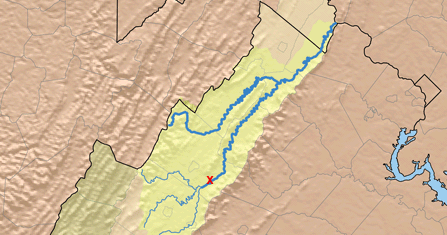
\includegraphics{../Figures-and-Maps/mcgaheysvilledam.png}
\caption{map of Neuse River}
\end{figure}

We are interested in both changes in physical process and changes in
chemical processes, which can vary widely according to the specific
river, its history, and the dam removal process (Foley et al 2017). Dams
allow for moderation of flow, often eliminating extreme flooding events.
Therefore, dam removal in combination with increasing extreme weather
events due to climate change could lead to more extreme and more
frequent high flow events. On the other hand, natural river systems and
riparian areas can be more resilient to flood events than artificially
constructed channels, so true restoration could help mitigate high flow
events to some extent.

Changes in water quality are also an area of interest. Large amounts of
sediment and minerals built up behind the dam may release quickly after
removal, especially if the removal was sudden rather than gradual (Foley
et al 2017). Over longer time, water quality is expected to improve
because of restored ecological processes.

\begin{enumerate}
\def\labelenumi{\arabic{enumi}.}
\item
  Question 1: Have discharge levels become more extreme since dam
  removal?
\item
  Question 2: Has there been an increase in release of sediment and
  nutrients over time?
\end{enumerate}

\begin{itemize}
\tightlist
\item
  Have levels steadily increased since dam removal, or did they spike
  and then stabilize?
\end{itemize}

\newpage

\hypertarget{dataset-information}{%
\section{Dataset Information}\label{dataset-information}}

The dataset consists of discharge and water quality data from stream
gage \#01631000, which is located on the South Fork of the Shenandoah
River downstream from the three dam removal sites. These data were
obtained from USGS StreamStats: \url{https://streamstats.usgs.gov/ss/}.

The dataset includes 183 parameters, but these parameters vary widely in
terms of how many datapoints were collected. To choose water quality
variables, I made a list of the top ten water quality parameters
according to the number of observations, and then selected three that I
thought would be particularly interesting and informative in light of
dam removal. These three were: suspended sediments, nitrogen, and
phosphate. Temperature is also included in the exploratory analyses. All
of these variables could be expected to change after dam removal.

\hypertarget{data-wrangling}{%
\subsection{Data Wrangling}\label{data-wrangling}}

The data were downloaded as two separate datasets: discharge
(`ShenaFlow') and water quality (`ShenaWQ'). Column names were changed
from defaults to be more comprehensible. Month and Year columns were
added to each dataset.

The discharge dataset was summarized into two dataframes, one by month
and the other by year. In both cases, discharge minimum, mean, and
maximum were calculated according to the summary unit.

The water quality dataset was transformed into a wider dataset with the
four parameters of interest divided into separate columns, instead of
being compiled in two columns by characteristic and value. The resulting
dataframe was also summarized by month, with minimum, mean, and maximum
calculated for each of the four parameters.

\begin{longtable}[]{@{}lrrrrrrrr@{}}
\toprule
& vars & n & mean & sd & min & max & range & se \\
\midrule
\endhead
Discharge & 1 & 33445 & 1602.856 & 2563.599 & 103 & 114000 & 113897 &
14.01795 \\
\bottomrule
\end{longtable}

\begin{longtable}[]{@{}lrrrrrrrr@{}}
\toprule
& vars & n & mean & sd & min & max & range & se \\
\midrule
\endhead
Nitrogen\_mg.L & 1 & 584 & 0.9911644 & 0.4509875 & 0.01 & 2.69 & 2.68 &
0.0186620 \\
Temp\_C & 2 & 767 & 14.2938722 & 8.2711759 & -0.10 & 30.50 & 30.60 &
0.2986549 \\
Phosphate\_mg.L & 3 & 579 & 0.2251330 & 0.2549664 & 0.00 & 1.93 & 1.93 &
0.0105960 \\
Sediments\_mg.L & 4 & 466 & 55.2227468 & 151.3406481 & 0.00 & 2020.00 &
2020.00 & 7.0107201 \\
\bottomrule
\end{longtable}

\newpage

\hypertarget{exploratory-analysis}{%
\section{Exploratory Analysis}\label{exploratory-analysis}}

Below are exploratory plots showing each parameter over time, with a
linear depiction of overall trend.

\begin{figure}
\centering
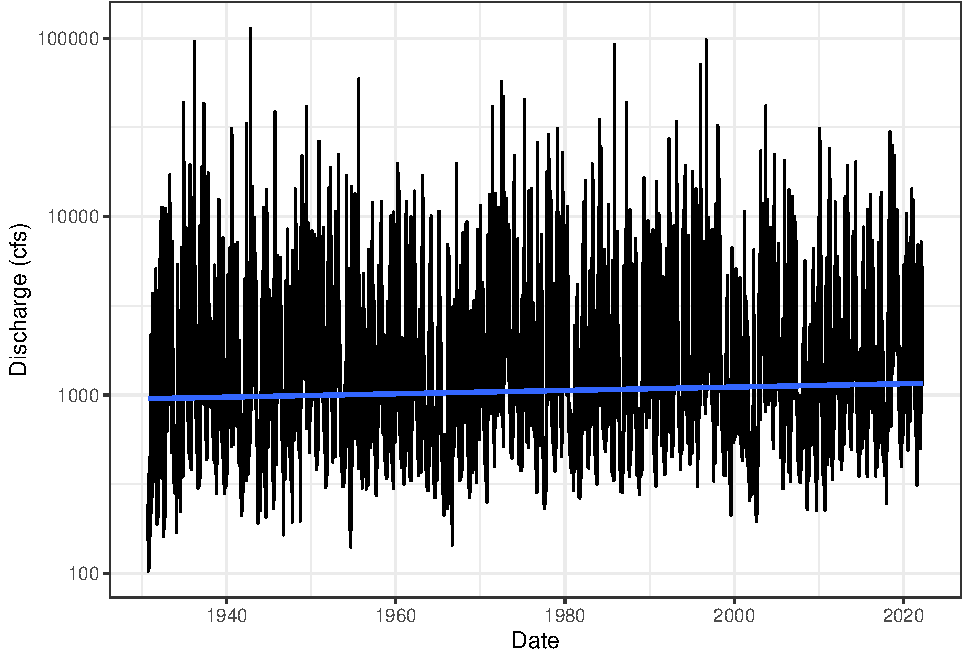
\includegraphics{Project_Template_files/figure-latex/exploration_plot1-1.pdf}
\caption{Discharge over time}
\end{figure}

\begin{figure}
\centering
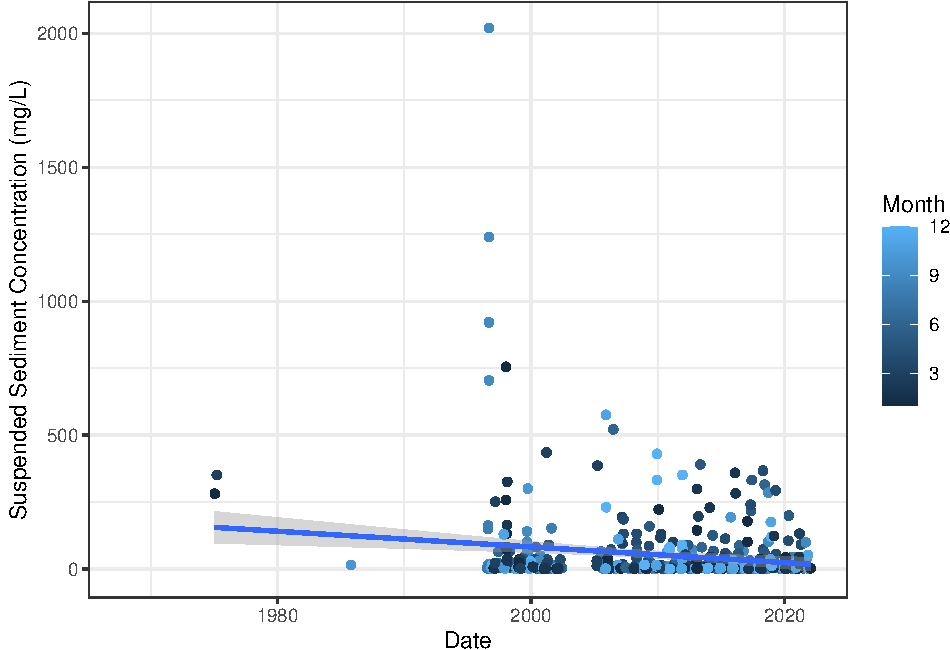
\includegraphics{Project_Template_files/figure-latex/exploration_plot2-1.pdf}
\caption{Sediment over time}
\end{figure}

\begin{figure}
\centering
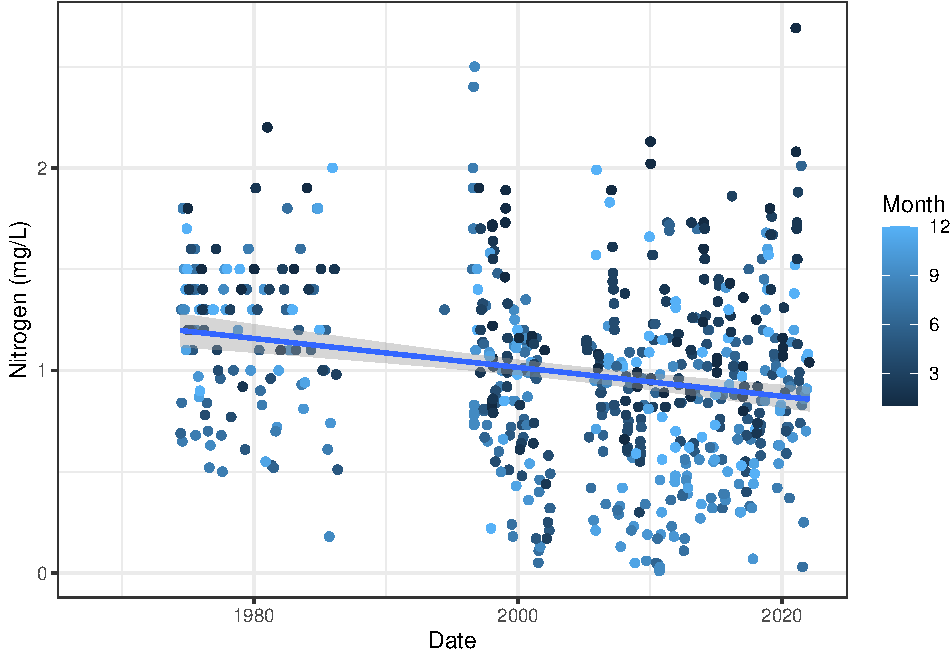
\includegraphics{Project_Template_files/figure-latex/exploration_plot3-1.pdf}
\caption{Nitrogen over time}
\end{figure}

\begin{figure}
\centering
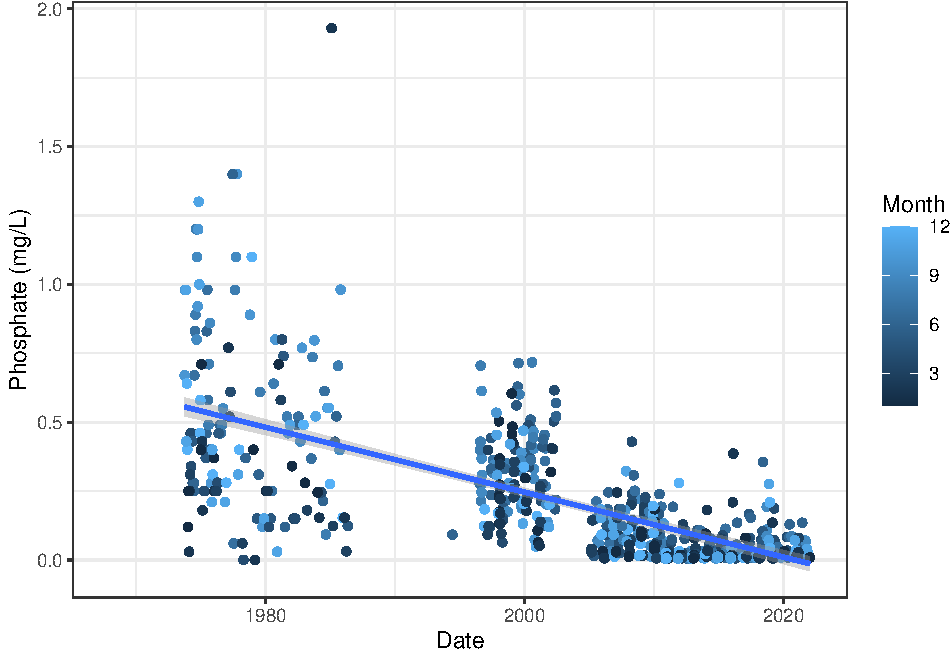
\includegraphics{Project_Template_files/figure-latex/exploration_plot4-1.pdf}
\caption{Phosphate over time}
\end{figure}

\begin{figure}
\centering
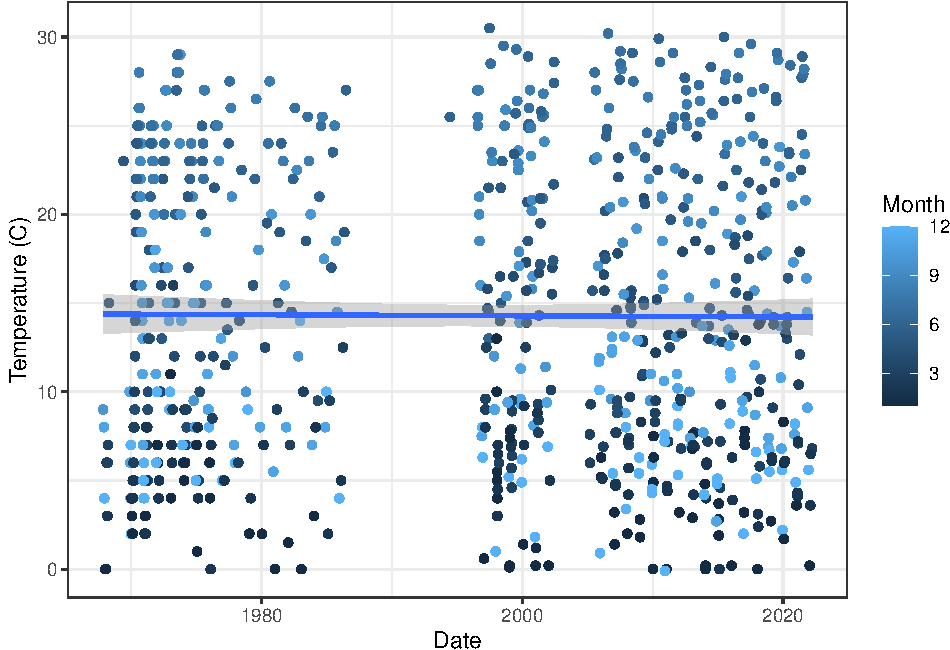
\includegraphics{Project_Template_files/figure-latex/exploration_plot5-1.pdf}
\caption{Temperature over time}
\end{figure}

\newpage

\hypertarget{analysis}{%
\section{Analysis}\label{analysis}}

\hypertarget{part-1}{%
\subsection{Part 1}\label{part-1}}

\begin{quote}
Question \#1: Have discharge extremes increased since the removal of the
dams? Has average discharge increased since dam removal?
\end{quote}

\begin{Shaded}
\begin{Highlighting}[]
\CommentTok{\# View monthly min and max flow over time}
\FunctionTok{ggplot}\NormalTok{(ShenaFlow\_monthly, }\FunctionTok{aes}\NormalTok{(}\AttributeTok{x =}\NormalTok{ Date)) }\SpecialCharTok{+}
  \FunctionTok{scale\_y\_log10}\NormalTok{() }\SpecialCharTok{+}
  \FunctionTok{geom\_line}\NormalTok{(}\FunctionTok{aes}\NormalTok{(}\AttributeTok{y =}\NormalTok{ Discharge\_min), }\AttributeTok{color =} \StringTok{"lightskyblue2"}\NormalTok{) }\SpecialCharTok{+}
  \FunctionTok{geom\_line}\NormalTok{(}\FunctionTok{aes}\NormalTok{(}\AttributeTok{y =}\NormalTok{ Discharge\_max), }\AttributeTok{color =} \StringTok{"steelblue3"}\NormalTok{) }\SpecialCharTok{+}
  \FunctionTok{geom\_vline}\NormalTok{(}\AttributeTok{xintercept =} \FunctionTok{as.numeric}\NormalTok{(}\FunctionTok{as.Date}\NormalTok{(}\StringTok{"2004{-}01{-}01"}\NormalTok{)), }
             \AttributeTok{linetype =} \DecValTok{4}\NormalTok{, }\AttributeTok{color =} \StringTok{"tomato4"}\NormalTok{) }\SpecialCharTok{+}
  \FunctionTok{labs}\NormalTok{(}\AttributeTok{x =} \StringTok{"Year"}\NormalTok{, }\AttributeTok{y =} \StringTok{"Discharge (cfs)"}\NormalTok{) }\SpecialCharTok{+}
  \FunctionTok{annotate}\NormalTok{(}\AttributeTok{geom =} \StringTok{"text"}\NormalTok{,}
           \AttributeTok{label =} \StringTok{"2004"}\NormalTok{,}
           \AttributeTok{x =} \FunctionTok{as.Date}\NormalTok{(}\StringTok{"2004{-}01{-}01"}\NormalTok{),}
           \AttributeTok{y =} \FunctionTok{as.numeric}\NormalTok{(}\DecValTok{100000}\NormalTok{),}
           \AttributeTok{angle =} \DecValTok{90}\NormalTok{, }
           \AttributeTok{vjust =} \DecValTok{2}\NormalTok{,}
           \AttributeTok{color =} \StringTok{"tomato4"}\NormalTok{)}
\end{Highlighting}
\end{Shaded}

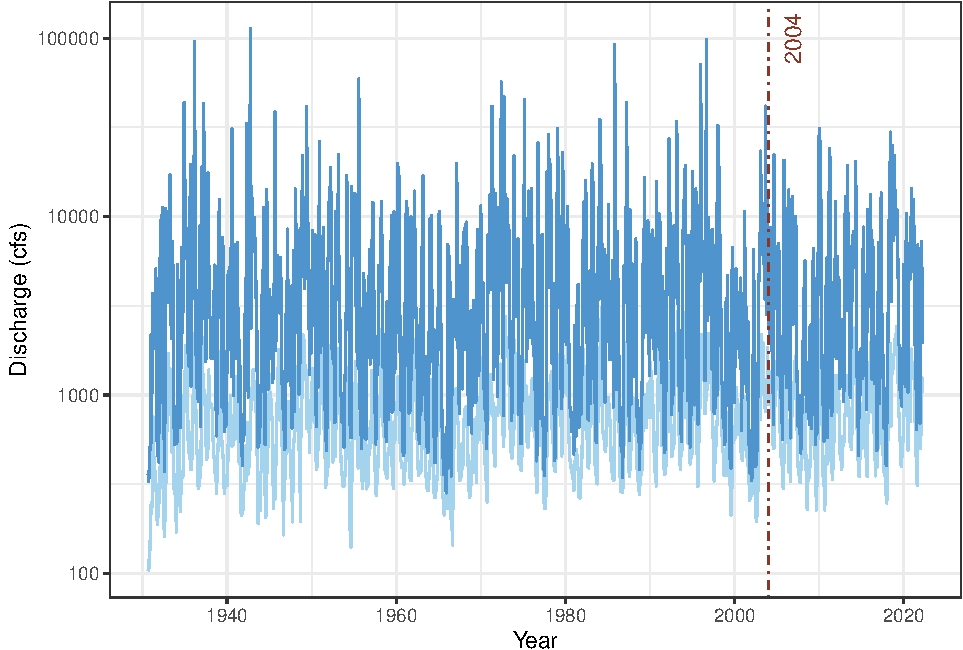
\includegraphics{Project_Template_files/figure-latex/Flow.analysis-1.pdf}

\begin{Shaded}
\begin{Highlighting}[]
\CommentTok{\# Extreme discharge does not appear to have increased. Check yearly to verify}

\CommentTok{\# View yearly min, max, mean flow over time}
\FunctionTok{ggplot}\NormalTok{(ShenaFlow\_yearly, }\FunctionTok{aes}\NormalTok{(}\AttributeTok{x =}\NormalTok{ Year)) }\SpecialCharTok{+}
  \FunctionTok{scale\_y\_log10}\NormalTok{() }\SpecialCharTok{+}
  \FunctionTok{geom\_line}\NormalTok{(}\FunctionTok{aes}\NormalTok{(}\AttributeTok{y =}\NormalTok{ Discharge\_min), }\AttributeTok{color =} \StringTok{"lightskyblue2"}\NormalTok{) }\SpecialCharTok{+}
  \FunctionTok{geom\_line}\NormalTok{(}\FunctionTok{aes}\NormalTok{(}\AttributeTok{y =}\NormalTok{ Discharge\_max), }\AttributeTok{color =} \StringTok{"steelblue"}\NormalTok{) }\SpecialCharTok{+}
  \FunctionTok{geom\_line}\NormalTok{(}\FunctionTok{aes}\NormalTok{(}\AttributeTok{y =}\NormalTok{ Discharge\_mean), }\AttributeTok{color =} \StringTok{"steelblue2"}\NormalTok{) }\SpecialCharTok{+}
  \FunctionTok{geom\_vline}\NormalTok{(}\AttributeTok{xintercept =} \FunctionTok{as.numeric}\NormalTok{(}\DecValTok{2004}\NormalTok{), }
             \AttributeTok{linetype =} \DecValTok{4}\NormalTok{, }\AttributeTok{color =} \StringTok{"tomato4"}\NormalTok{) }\SpecialCharTok{+}
  \FunctionTok{labs}\NormalTok{(}\AttributeTok{y =} \StringTok{"Discharge (cfs)"}\NormalTok{) }\SpecialCharTok{+}
  \FunctionTok{annotate}\NormalTok{(}\AttributeTok{geom =} \StringTok{"text"}\NormalTok{,}
           \AttributeTok{label =} \StringTok{"2004"}\NormalTok{,}
           \AttributeTok{x =} \FunctionTok{as.numeric}\NormalTok{(}\DecValTok{2004}\NormalTok{),}
           \AttributeTok{y =} \FunctionTok{as.numeric}\NormalTok{(}\DecValTok{100000}\NormalTok{),}
           \AttributeTok{angle =} \DecValTok{90}\NormalTok{, }
           \AttributeTok{vjust =} \DecValTok{2}\NormalTok{,}
           \AttributeTok{color =} \StringTok{"tomato4"}\NormalTok{)}
\end{Highlighting}
\end{Shaded}

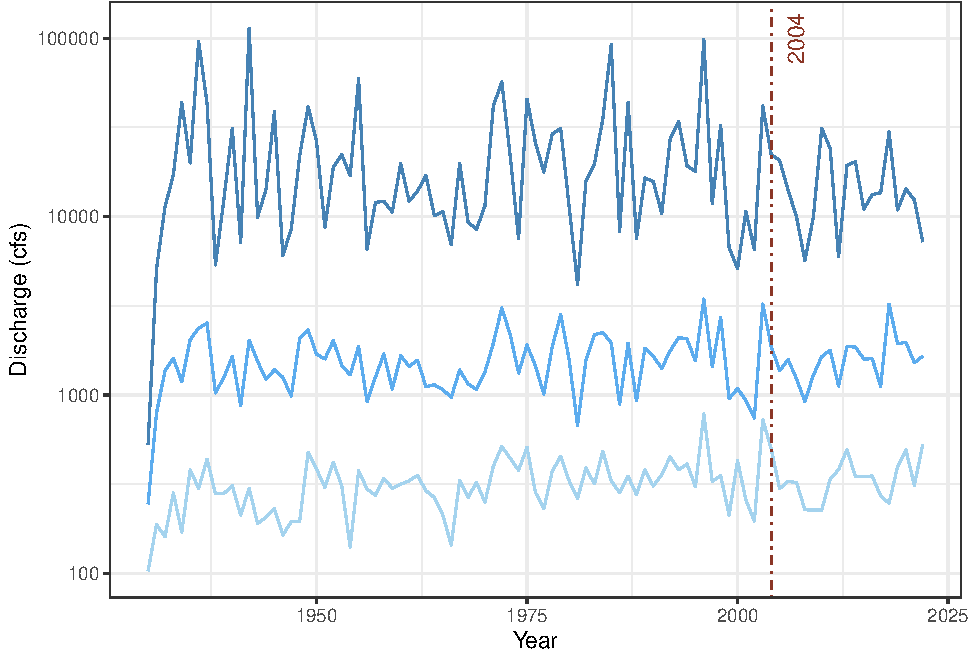
\includegraphics{Project_Template_files/figure-latex/Flow.analysis-2.pdf}

\begin{Shaded}
\begin{Highlighting}[]
\CommentTok{\# Yes, extremes appear smaller since the dam removal}

\CommentTok{\# Create before and after datasets}
\NormalTok{ShenaFlow.before }\OtherTok{\textless{}{-}}\NormalTok{ ShenaFlow[ShenaFlow}\SpecialCharTok{$}\NormalTok{Date }\SpecialCharTok{\textless{}} \StringTok{"2004{-}01{-}01"}\NormalTok{,]}
\NormalTok{ShenaFlow.after }\OtherTok{\textless{}{-}}\NormalTok{ ShenaFlow[ShenaFlow}\SpecialCharTok{$}\NormalTok{Date }\SpecialCharTok{\textgreater{}=} \StringTok{"2006{-}01{-}01"}\NormalTok{,]}

\CommentTok{\# Create summary table to compare before and after dam removal}
\NormalTok{before\_summary }\OtherTok{\textless{}{-}} \FunctionTok{describe}\NormalTok{(ShenaFlow.before[,}\StringTok{"Discharge"}\NormalTok{], }\AttributeTok{fast =}\NormalTok{ T)}
\NormalTok{after\_summary }\OtherTok{\textless{}{-}} \FunctionTok{describe}\NormalTok{(ShenaFlow.after[,}\StringTok{"Discharge"}\NormalTok{], }\AttributeTok{fast =}\NormalTok{ T)}
\NormalTok{flow\_summary }\OtherTok{\textless{}{-}} \FunctionTok{rbind}\NormalTok{(before\_summary, after\_summary)}
\CommentTok{\# rename columns}
\NormalTok{flow\_summary}\SpecialCharTok{$}\NormalTok{vars }\OtherTok{\textless{}{-}} \FunctionTok{c}\NormalTok{(}\StringTok{"Before"}\NormalTok{, }\StringTok{"After"}\NormalTok{)}
\FunctionTok{colnames}\NormalTok{(flow\_summary)[}\DecValTok{1}\NormalTok{] }\OtherTok{\textless{}{-}} \StringTok{"Timeframe Relative to Dam Removal"}

\CommentTok{\# Print summary table}
\FunctionTok{kable}\NormalTok{(flow\_summary, }\AttributeTok{caption =} \StringTok{"Summary Statistics for Discharge"}\NormalTok{)}
\end{Highlighting}
\end{Shaded}

\begin{longtable}[]{@{}llrrrrrrr@{}}
\caption{Summary Statistics for Discharge}\tabularnewline
\toprule
& Timeframe Relative to Dam Removal & n & mean & sd & min & max & range
& se \\
\midrule
\endfirsthead
\toprule
& Timeframe Relative to Dam Removal & n & mean & sd & min & max & range
& se \\
\midrule
\endhead
X1 & Before & 26764 & 1594.155 & 2687.319 & 103 & 114000 & 113897 &
16.42645 \\
X11 & After & 5950 & 1640.134 & 2010.450 & 226 & 31300 & 31074 &
26.06362 \\
\bottomrule
\end{longtable}

\begin{Shaded}
\begin{Highlighting}[]
\CommentTok{\# It appears that average flow may be higher since the dam removal}
\CommentTok{\# Test with a t{-}test}
\NormalTok{t.test\_before.after }\OtherTok{\textless{}{-}} \FunctionTok{t.test}\NormalTok{(ShenaFlow.before}\SpecialCharTok{$}\NormalTok{Discharge, ShenaFlow.after}\SpecialCharTok{$}\NormalTok{Discharge, }\AttributeTok{var.equal =} \ConstantTok{FALSE}\NormalTok{)}
\NormalTok{t.test\_before.after}
\end{Highlighting}
\end{Shaded}

\begin{verbatim}
## 
##  Welch Two Sample t-test
## 
## data:  ShenaFlow.before$Discharge and ShenaFlow.after$Discharge
## t = -1.4925, df = 11220, p-value = 0.1356
## alternative hypothesis: true difference in means is not equal to 0
## 95 percent confidence interval:
##  -106.36901   14.40966
## sample estimates:
## mean of x mean of y 
##  1594.155  1640.134
\end{verbatim}

\begin{Shaded}
\begin{Highlighting}[]
\CommentTok{\# Not statistically different}
\end{Highlighting}
\end{Shaded}

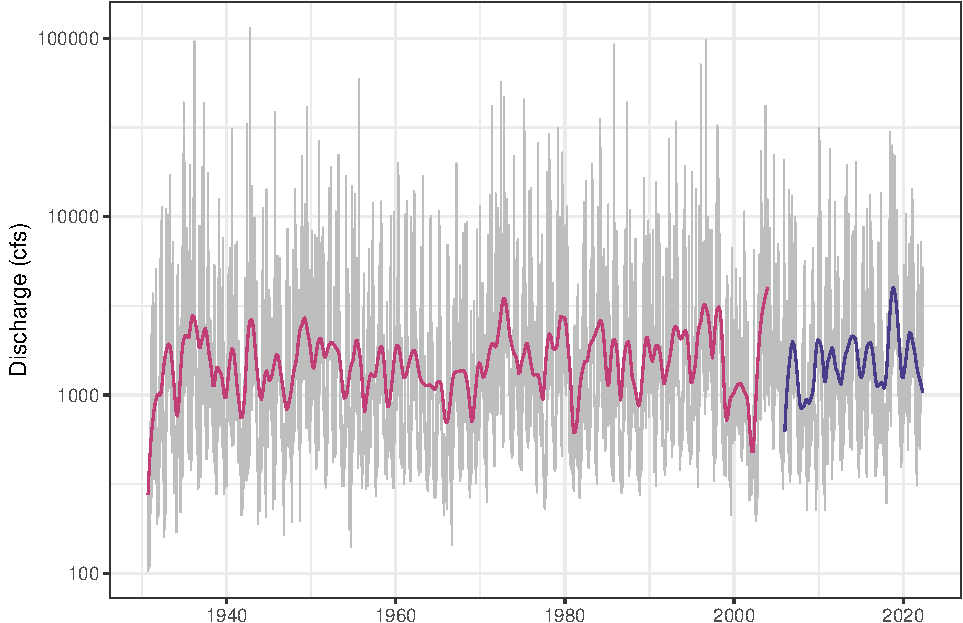
\includegraphics{Project_Template_files/figure-latex/flow_ts_graph-1.pdf}

\newpage

\hypertarget{part-2}{%
\subsection{Part 2}\label{part-2}}

\begin{quote}
Question \#2: Has there been an increase in release of sediment and
nutrients over time? + Have levels increased since dam removal, or did
they spike and then stabilize?
\end{quote}

\hypertarget{sediment}{%
\subsubsection{Sediment}\label{sediment}}

\begin{Shaded}
\begin{Highlighting}[]
\CommentTok{\# Re{-}examine data, excluding small number of early points and rescaling}
\FunctionTok{ggplot}\NormalTok{(}\AttributeTok{data =}\NormalTok{ ShenaWQ\_processed[ShenaWQ\_processed}\SpecialCharTok{$}\NormalTok{Date }\SpecialCharTok{\textgreater{}} \StringTok{"1995{-}01{-}01"}\NormalTok{,], }
             \FunctionTok{aes}\NormalTok{(}\AttributeTok{x =}\NormalTok{ Date, }\AttributeTok{y =}\NormalTok{ Sediments\_mg.L, }\AttributeTok{color =}\NormalTok{ Month)) }\SpecialCharTok{+}
  \FunctionTok{geom\_point}\NormalTok{() }\SpecialCharTok{+}
  \FunctionTok{geom\_smooth}\NormalTok{(}\AttributeTok{method =} \StringTok{"lm"}\NormalTok{) }\SpecialCharTok{+}
  \FunctionTok{scale\_y\_log10}\NormalTok{() }
\end{Highlighting}
\end{Shaded}

\begin{verbatim}
## Warning: Transformation introduced infinite values in continuous y-axis

## Warning: Transformation introduced infinite values in continuous y-axis
\end{verbatim}

\begin{verbatim}
## `geom_smooth()` using formula 'y ~ x'
\end{verbatim}

\begin{verbatim}
## Warning: Removed 21 rows containing non-finite values (stat_smooth).
\end{verbatim}

\begin{verbatim}
## Warning: Removed 18 rows containing missing values (geom_point).
\end{verbatim}

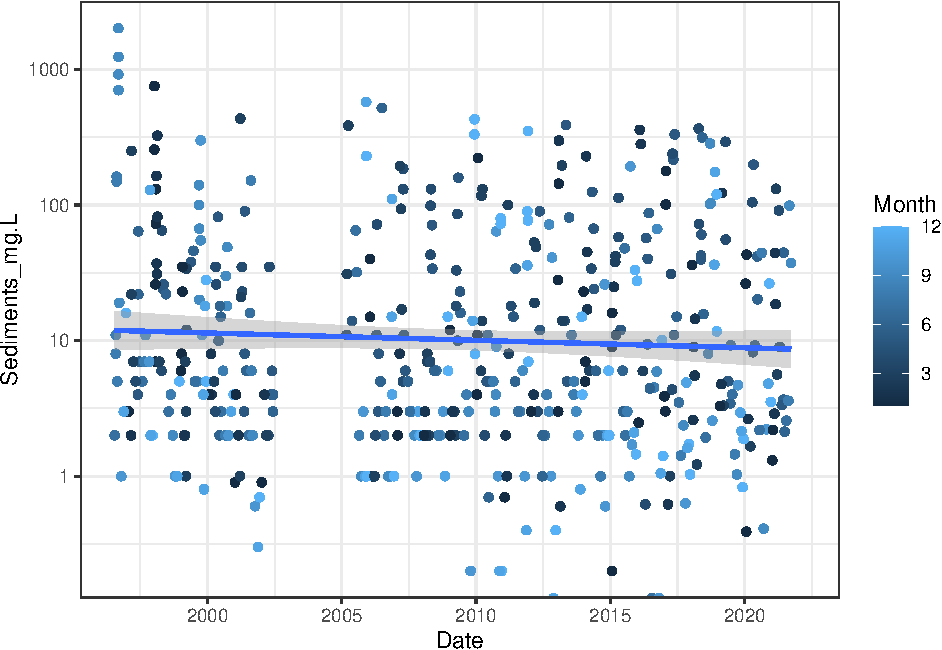
\includegraphics{Project_Template_files/figure-latex/Sediment_Analysis-1.pdf}

\begin{Shaded}
\begin{Highlighting}[]
\CommentTok{\# Create before and after WQ datasets}
\NormalTok{ShenaWQ.before }\OtherTok{\textless{}{-}}\NormalTok{ ShenaWQ\_processed[ShenaWQ\_processed}\SpecialCharTok{$}\NormalTok{Date }\SpecialCharTok{\textless{}} \StringTok{"2004{-}01{-}01"}\NormalTok{,]}
\NormalTok{ShenaWQ.after }\OtherTok{\textless{}{-}}\NormalTok{ ShenaWQ\_processed[ShenaWQ\_processed}\SpecialCharTok{$}\NormalTok{Date }\SpecialCharTok{\textgreater{}=} \StringTok{"2006{-}01{-}01"}\NormalTok{,]}

\CommentTok{\# Test whether average sediment varied before versus after dam removal}
\NormalTok{t.test\_sediment }\OtherTok{\textless{}{-}} \FunctionTok{t.test}\NormalTok{(ShenaWQ.before}\SpecialCharTok{$}\NormalTok{Sediments\_mg.L, ShenaWQ.after}\SpecialCharTok{$}\NormalTok{Sediments\_mg.L, }\AttributeTok{var.equal =} \ConstantTok{FALSE}\NormalTok{)}
\NormalTok{t.test\_sediment}
\end{Highlighting}
\end{Shaded}

\begin{verbatim}
## 
##  Welch Two Sample t-test
## 
## data:  ShenaWQ.before$Sediments_mg.L and ShenaWQ.after$Sediments_mg.L
## t = 1.9798, df = 148.99, p-value = 0.04957
## alternative hypothesis: true difference in means is not equal to 0
## 95 percent confidence interval:
##   0.08085757 84.02230236
## sample estimates:
## mean of x mean of y 
##  83.15474  41.10316
\end{verbatim}

\begin{Shaded}
\begin{Highlighting}[]
\CommentTok{\# Sediment levels were significantly lower post (p = 0.050)}
\CommentTok{\# Not possible to see whether there was a spike immediately after dam }
\CommentTok{\# removal because of gap in data}
\end{Highlighting}
\end{Shaded}

\newpage

\hypertarget{nitrogen}{%
\subsubsection{Nitrogen}\label{nitrogen}}

Have ni

\begin{Shaded}
\begin{Highlighting}[]
\CommentTok{\# Re{-}examine data, zoomed in}
\FunctionTok{ggplot}\NormalTok{(ShenaWQ\_processed, }\FunctionTok{aes}\NormalTok{(}\AttributeTok{x =}\NormalTok{ Date, }\AttributeTok{y =}\NormalTok{ Nitrogen\_mg.L)) }\SpecialCharTok{+}
  \FunctionTok{geom\_point}\NormalTok{(}\FunctionTok{aes}\NormalTok{(}\AttributeTok{color =}\NormalTok{ Month)) }\SpecialCharTok{+}
  \FunctionTok{geom\_smooth}\NormalTok{(}\AttributeTok{method =} \StringTok{"lm"}\NormalTok{) }\SpecialCharTok{+}
  \FunctionTok{scale\_x\_date}\NormalTok{(}\AttributeTok{limits =} \FunctionTok{c}\NormalTok{(}\FunctionTok{as.Date}\NormalTok{(}\StringTok{"1972{-}01{-}01"}\NormalTok{), }
                          \FunctionTok{as.Date}\NormalTok{(}\StringTok{"2022{-}02{-}17"}\NormalTok{)))}
\end{Highlighting}
\end{Shaded}

\begin{verbatim}
## `geom_smooth()` using formula 'y ~ x'
\end{verbatim}

\begin{verbatim}
## Warning: Removed 190 rows containing non-finite values (stat_smooth).
\end{verbatim}

\begin{verbatim}
## Warning: Removed 190 rows containing missing values (geom_point).
\end{verbatim}

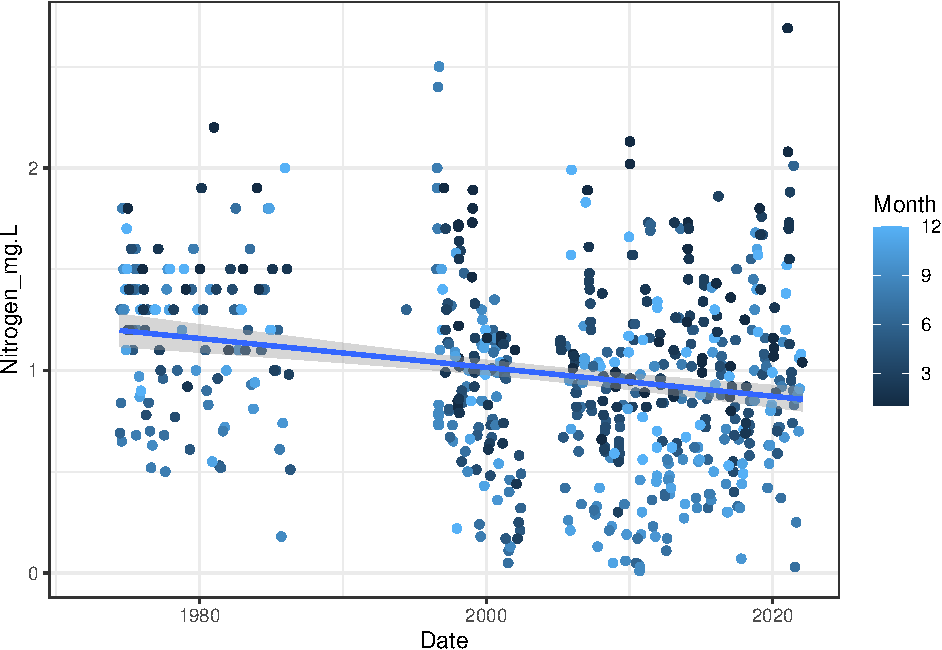
\includegraphics{Project_Template_files/figure-latex/Nitrogen_Analysis-1.pdf}

\begin{Shaded}
\begin{Highlighting}[]
\CommentTok{\# Create yearly summary table to visualize differently}
\NormalTok{ShenaWQ\_yearly }\OtherTok{\textless{}{-}}\NormalTok{ ShenaWQ\_processed }\SpecialCharTok{\%\textgreater{}\%}
  \FunctionTok{group\_by}\NormalTok{(Year) }\SpecialCharTok{\%\textgreater{}\%}
  \FunctionTok{summarise}\NormalTok{(}\AttributeTok{Nitrogen\_min =} \FunctionTok{min}\NormalTok{(Nitrogen\_mg.L),}
            \AttributeTok{Nitrogen\_max =} \FunctionTok{max}\NormalTok{(Nitrogen\_mg.L),}
            \AttributeTok{Nitrogen\_mean =} \FunctionTok{mean}\NormalTok{(Nitrogen\_mg.L)) }\SpecialCharTok{\%\textgreater{}\%}
  \FunctionTok{filter}\NormalTok{(Year }\SpecialCharTok{\textgreater{}=} \DecValTok{1972}\NormalTok{)}

\CommentTok{\# Plot results}
\FunctionTok{ggplot}\NormalTok{(ShenaWQ\_yearly, }\FunctionTok{aes}\NormalTok{(}\AttributeTok{x =}\NormalTok{ Year)) }\SpecialCharTok{+}
  \FunctionTok{geom\_line}\NormalTok{(}\FunctionTok{aes}\NormalTok{(}\AttributeTok{y =}\NormalTok{ Nitrogen\_min), }\AttributeTok{color =} \StringTok{"darkgoldenrod2"}\NormalTok{) }\SpecialCharTok{+}
  \FunctionTok{geom\_line}\NormalTok{(}\FunctionTok{aes}\NormalTok{(}\AttributeTok{y =}\NormalTok{ Nitrogen\_max), }\AttributeTok{color =} \StringTok{"coral4"}\NormalTok{) }\SpecialCharTok{+}
  \FunctionTok{geom\_line}\NormalTok{(}\FunctionTok{aes}\NormalTok{(}\AttributeTok{y =}\NormalTok{ Nitrogen\_mean), }\AttributeTok{color =} \StringTok{"chocolate"}\NormalTok{) }\SpecialCharTok{+}
  \FunctionTok{labs}\NormalTok{(}\AttributeTok{y =} \StringTok{"Nitrogen (mg/L)"}\NormalTok{)}
\end{Highlighting}
\end{Shaded}

\begin{verbatim}
## Warning: Removed 6 row(s) containing missing values (geom_path).
\end{verbatim}

\begin{verbatim}
## Warning: Removed 6 row(s) containing missing values (geom_path).

## Warning: Removed 6 row(s) containing missing values (geom_path).
\end{verbatim}

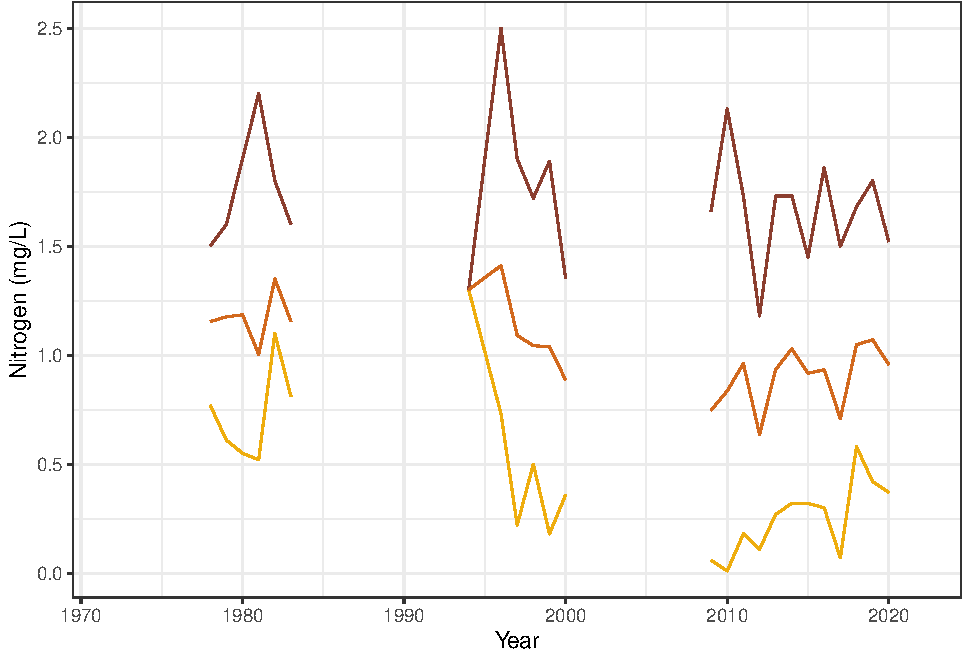
\includegraphics{Project_Template_files/figure-latex/Nitrogen_Analysis-2.pdf}

\begin{Shaded}
\begin{Highlighting}[]
\CommentTok{\# Test whether average sediment varied before versus after dam removal}
\NormalTok{t.test\_nitrogen }\OtherTok{\textless{}{-}} \FunctionTok{t.test}\NormalTok{(ShenaWQ.before}\SpecialCharTok{$}\NormalTok{Nitrogen\_mg.L, ShenaWQ.after}\SpecialCharTok{$}\NormalTok{Nitrogen\_mg.L, }\AttributeTok{var.equal =} \ConstantTok{FALSE}\NormalTok{)}
\NormalTok{t.test\_nitrogen}
\end{Highlighting}
\end{Shaded}

\begin{verbatim}
## 
##  Welch Two Sample t-test
## 
## data:  ShenaWQ.before$Nitrogen_mg.L and ShenaWQ.after$Nitrogen_mg.L
## t = 4.5603, df = 550.8, p-value = 0.000006299
## alternative hypothesis: true difference in means is not equal to 0
## 95 percent confidence interval:
##  0.0961950 0.2417647
## sample estimates:
## mean of x mean of y 
## 1.0861811 0.9172013
\end{verbatim}

\begin{Shaded}
\begin{Highlighting}[]
\CommentTok{\# Sediment levels were significantly lower post (p \textless{} 0.001)}
\CommentTok{\# Not possible to see whether there was a spike immediately after dam }
\CommentTok{\# removal because of gap in data}
\end{Highlighting}
\end{Shaded}

\newpage

\hypertarget{summary-and-conclusions}{%
\section{Summary and Conclusions}\label{summary-and-conclusions}}

\newpage

\hypertarget{references}{%
\section{References}\label{references}}

\begin{itemize}
\tightlist
\item
  Foley, M. M., J. R. Bellmore, J. E. O'Connor, J. J. Duda, A. E. East,
  G. E. Grant, C. W. Anderson, J. A. Bountry, M. J. Collins, P. J.
  Connolly, L. S. Craig, J. E. Evans, S. L. Greene,F. J. Magilligan, C.
  S. Magirl, J. J. Major, G. R. Pess,T. J. Randle, P. B. Shafroth, C. E.
  Torgersen, D. Tullos, A. C. Wilcox. 2017. Dam removal: Listening in.
  Water Resources Research. 53(7):5229-5246.
  \url{https://doi-org.proxy.lib.duke.edu/10.1002/2017WR020457}
\end{itemize}

Map source:
\url{http://www.virginiaplaces.org/watersheds/fishpassage.html}

Sediment deposits alter downstream tidal communities
\url{https://journals.plos.org/plosone/article?id=10.1371/journal.pone.0187742\#references}

info: \url{https://dwr.virginia.gov/fishing/fish-passage/\#orange}

\end{document}
